%!TEX root = ../dissertation.tex
\newpage

% If you do want an image in the colophon:
% \begin{figure}
%   \vspace{20pt}
%   \centering
%   \hspace*{-32pt}
%   % 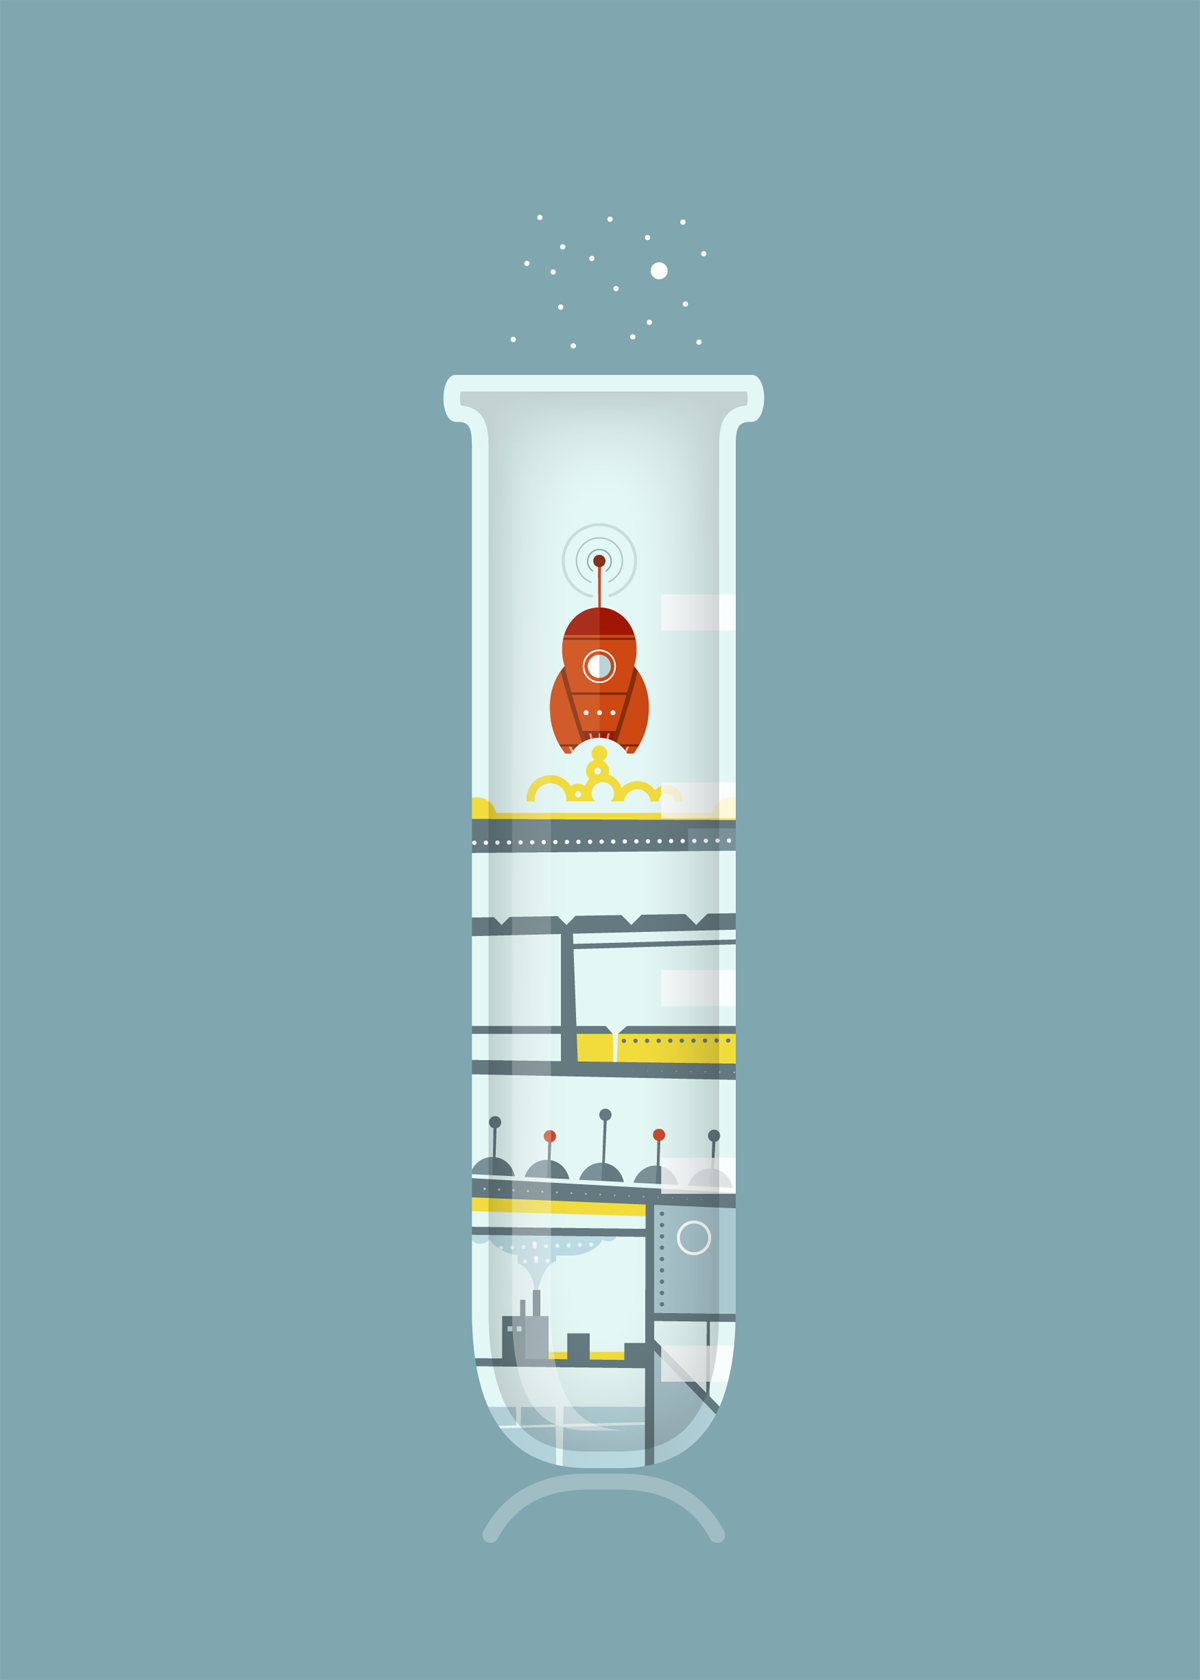
\includegraphics[width=0.4\textwidth]{endmatter/colophon.png}
% \end{figure}

% % If you don't want an image in the colophon:
% % \vspace*{200pt}

% \begin{center}
% \parbox{205pt}{\lettrine[lines=2,slope=-2pt,findent=4pt, nindent=0pt]{\textcolor{SchoolColor}{T}}{his report was typeset} using \LaTeX, originally developed by Leslie Lamport and based on Donald Knuth's \TeX. The body text is 11 point \href{https://github.com/georgd/EB-Garamond}{EB-Garamond}. A special thanks to Jordan Suchow for supplying this template under an open source license. Others looking for a similar look \& feel should review his \href{https://github.com/suchow/Dissertate}{github project}.}
% \end{center}
